\documentclass{beamer}

\usepackage[utf8]{inputenc}
\usepackage{color}
\usepackage{amsfonts}	% Real
\usepackage{bm}		% bold math symbols
\usepackage{amsmath}

\usepackage{booktabs} % eleganckie tabelki


\usetheme{boxes}      % Wybór tematu wyglądu, gdy chcemy inny
%\usecolortheme{rose}   % Wybór tematu kolorystycznego, j.w.

%Konfiguracja dla pakietu hyperref:
\hypersetup{
  unicode=true,           % włączenie wyświetlania pliterek w zakładkach
%  pdfpagemode=FullScreen, % włączenie trybu pełnoekranowanego
  pdfsubject=Graph Neural Networks,      % temat prezentacji
  pdfkeywords={gnn, graph neural network, graph, classification} % slowa kluczowe
}

%% Dane do strony tytułowej
\author{Aleksy Barcz}
\title{Fast learning method for RAAM based on sensitivity analysis}
\date{\today}
\institute{Warsaw University of Technology}

\setbeamercovered{transparent}

\begin{document}
\frame{\titlepage}

\begin{frame}
\frametitle{Graph-oriented neural networks}
\begin{columns}
	\begin{column}{0.66\textwidth}
		\begin{itemize}
			\item graph structure processed directly
			\item build meaningful representation
			\item classification and regression
			\item based on feed-forward neural networks
		\end{itemize}
	\end{column}
	\begin{column}{0.34\textwidth}
		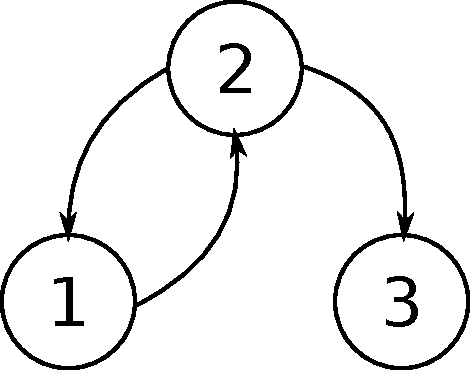
\includegraphics[scale=0.4]{img/graph}
	\end{column}
\end{columns}
\end{frame}

\begin{frame}
\frametitle{Recursive Auto-Associative Memory}
\begin{columns}
	\begin{column}{0.6\textwidth}
		\begin{itemize}
			\item coder + decoder
			\item graph $\Rightarrow$ root representation
			\item coder: encode nodes bottom-up
			\item decoder: decode top-down
		\end{itemize}
	\end{column}
	\begin{column}{0.4\textwidth}
		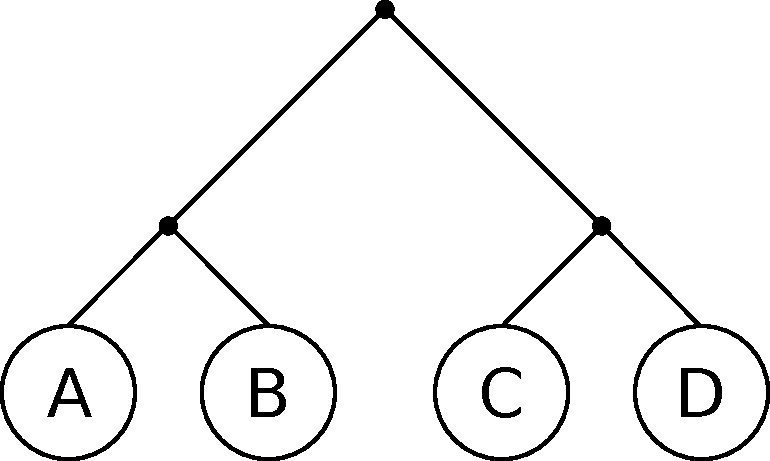
\includegraphics[scale=0.35]{img/tree_for_raam}
	\end{column}
\end{columns}
\end{frame}

\begin{frame}
\frametitle{RAAM training}
\begin{columns}
	\begin{column}{0.66\textwidth}
		\begin{itemize}
			\item coder + decoder = multilayer FNN
			\item standard backpropagation / unfolded network
			\item $O(10^2)..O(10^3)$ iterations
		\end{itemize}
	\end{column}
	\begin{column}{0.34\textwidth}
		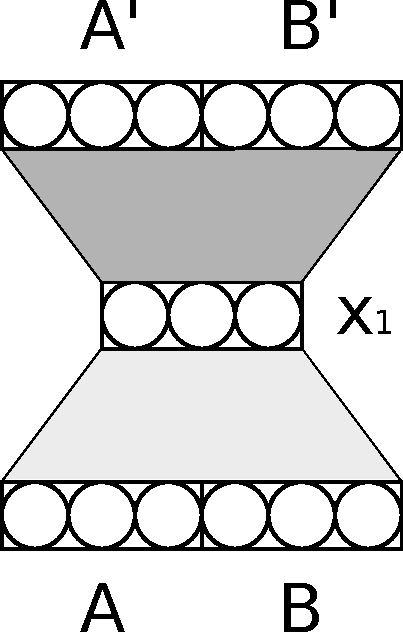
\includegraphics[scale=0.4]{img/raam_single}
	\end{column}
\end{columns}
\end{frame}

\begin{frame}
\frametitle{Sensitivity Based Linear Learning Machine}
\begin{center}
	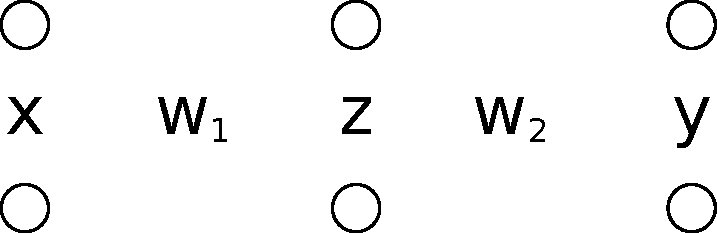
\includegraphics[scale=0.5]{img/fnn}
\end{center}
\end{frame}

\begin{frame}
\frametitle{Backpropagation vs SBLLM}
\begin{center}
	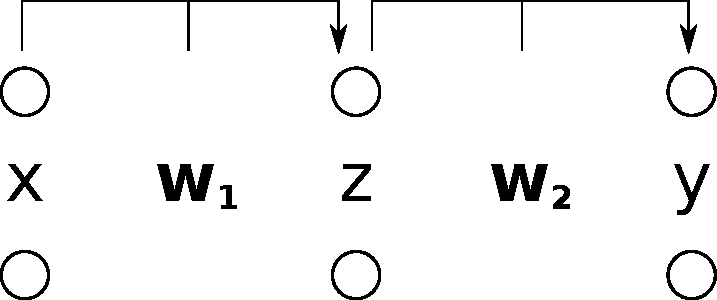
\includegraphics[scale=0.5]{img/fnn_bp}
	\vspace{1.5cm}
	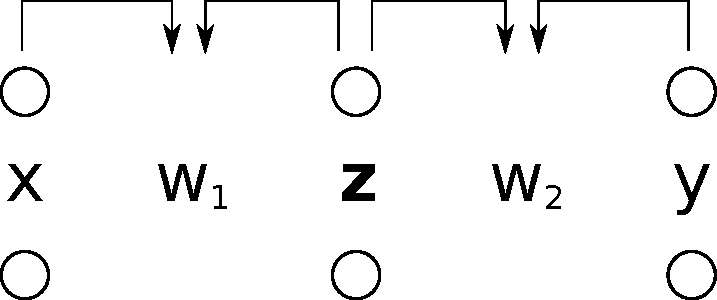
\includegraphics[scale=0.5]{img/fnn_sbllm}
\end{center}
\end{frame}

\begin{frame}
\frametitle{SBLLM for FNN}
\begin{itemize}
	\item fast training (1-2 iterations)
	\item more hidden neurons needed
	\item sensitive to low-dimensional data
\end{itemize}
\end{frame}

\begin{frame}
\frametitle{SBLLM + RAAM}
\begin{itemize}
	\item syntactic trees clustering problem
	\item 15 trees, 5 phrase types
	\item ((D (A N)) (V (P (D N))))
\end{itemize}
\end{frame}

\begin{frame}
\frametitle{SBLLM + RAAM}
\begin{itemize}
	\item 4-5 iterations instead of hundreds
	\item same number of hidden neurons needed
	\item good precision
	\item similar results to the original paper
\end{itemize}
\end{frame}

\begin{frame}
\frametitle{Sentence clustering}
\begin{center}
	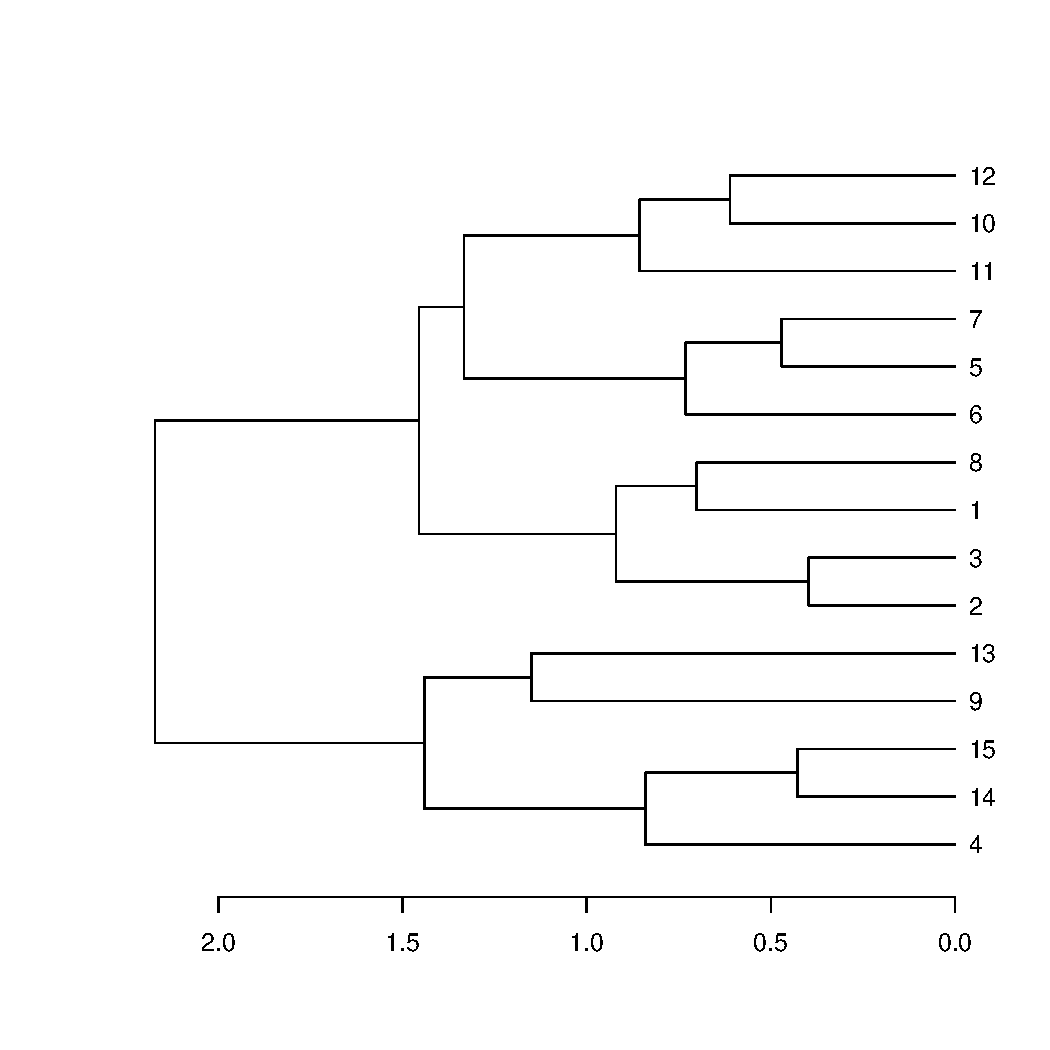
\includegraphics[scale=0.5]{img/raam-sbllm-syntax}
\end{center}
\end{frame}

\begin{frame}
\begin{center}
\Huge{\emph{Thank you}}
\end{center}
\end{frame}

\begin{frame}

\begin{equation}
y_{js} = f^{(2)}_j \left( w^{(2)}_{j0} + \sum_{k=1}^{K} w^{(2)}_{jk} z_{ks}\right); \quad j = 1,2,...,J; \quad s = 1,2,...,S.
\label{eq:threelayer2}
\end{equation}

\begin{equation}
z_{ks} = f^{(1)}_k \left( w^{(1)}_{k0} + \sum_{i=1}^{I}w^{(1)}_{ki}x_{is} \right); \quad k = 1,2,...,K; \quad s = 1,2,...,S.
\label{eq:threelayer1}
\end{equation}

\end{frame}

\begin{frame}

\begin{align*}
Q = Q^{(1)} + Q^{(2)}
&= \sum_{s=1}^{S}\sum_{k=1}^{K} \left( \sum_{i=1}^{I} w^{(1)}_{ki} x_{is} - f^{(1)^{-1}}_k(z_{ks}) \right)^{2}\\
&+ \sum_{s=1}^{S}\sum_{j=1}^{J} \left( \sum_{k=1}^{K} w^{(2)}_{jk} z_{ks} - f^{(2)^{-1}}_j(d_{js}) \right)^{2}.
\label{eq:qall}
\end{align*}

\begin{equation}
Q(\bm{z} + \Delta \bm{z}) = Q(\bm{z}) + \sum_{k=1}^{K}\sum_{s=1}^{S} \frac{\partial Q(\bm{z})}{\partial z_{ks}} \Delta z_{ks} \approx 0.
\label{eq:qdz}
\end{equation}
\end{frame}


\begin{frame}
\frametitle{History - the GNN branch}
\begin{enumerate}
	\item RAAM - trees, leaf labels
	\item LRAAM - trees, node labels
	\item GNN - graphs, node and edge labels
\end{enumerate}
\end{frame}

\end{document}
